\section{Feature matching}

\subsection{Question 1 (on increasing the threshold ratio)}

{\bfseries Modify the previous threshold. What is the effect of this
threshold? Comment your response.\\[.5cm]}

We can see the result of the default matching process in figure \ref{fig:matching15thres}.

\begin{figure}[htb]
	\centering
		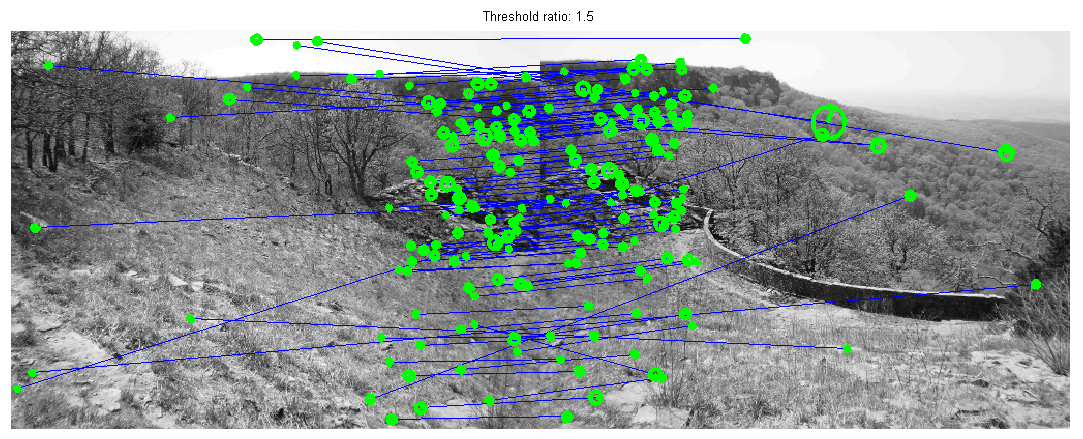
\includegraphics[width=\textwidth]{./img/ex1/matching_15_thres.png}
	\caption{Result of matching with a threshold ratio of 1.5 (default)}
	\label{fig:matching15thres}
\end{figure}

We have also computed the matches using different thresholds. In figure
\ref{fig:matching20thres} we can see the result of the matching algorithm
with a threshold ratio of 2.0. It is clear that there are fewer matches. This is
due to the fact that the ratio between the distances to the first and second best
matches acts as an uniqueness measure. Therefore increasing the threshold leads
to a more restrictive selection of the relevant matches and to a lower number of
matches at the end. In other words, since we consider just the matches that
accomplish $ \frac{d_2}{d_1} \geq THR $ (being $ d_1 $ and $ d_2 $ the distances
to the closest and second closest correspondences), a higher value of THR filters
out matches with a ratio $ \frac{d_2}{d_1} $ closer to 1.

\begin{figure}[htb]
	\centering
		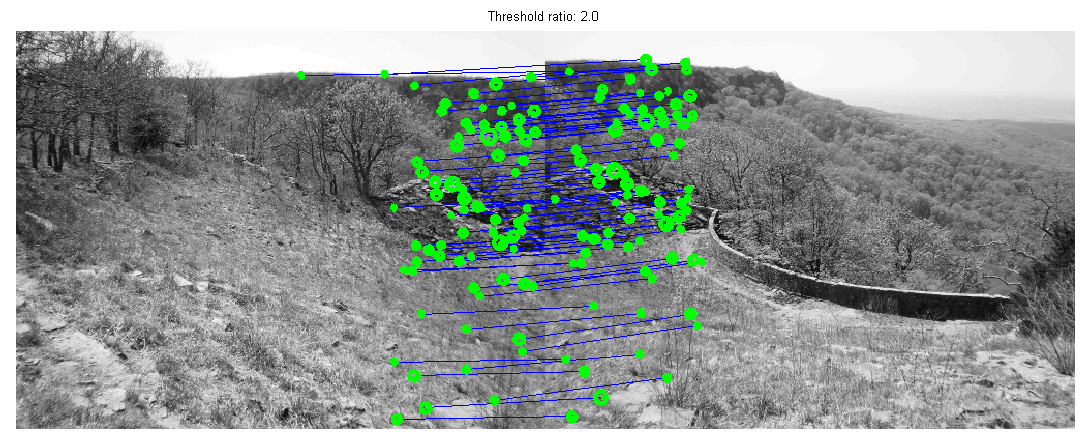
\includegraphics[width=\textwidth]{./img/ex1/matching_20_thres.png}
	\caption{Result of matching with a threshold ratio of 2.0}
	\label{fig:matching20thres}
\end{figure}

On the other hand the effect is reverted when we reduce the threshold. In figure
\ref{fig:matching10thres} we can see that there is a very notable increment in
the number of matches when we set the threshold to 1.0.

\begin{figure}[htb]
	\centering
		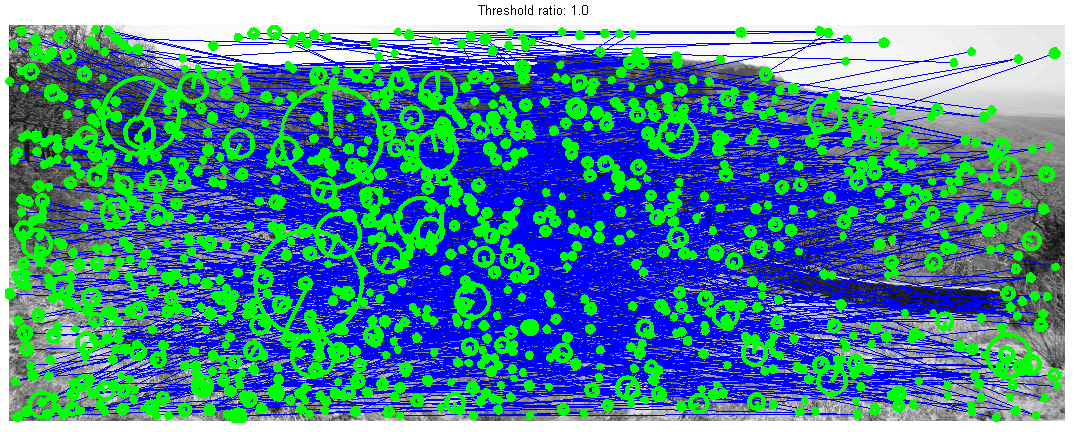
\includegraphics[width=\textwidth]{./img/ex1/matching_10_thres.png}
	\caption{Result of matching with a threshold ratio of 1.0}
	\label{fig:matching10thres}
\end{figure}

\subsection{Question 2 (on introducing a linear model)}

{\bfseries Comment on the obtained result. Is the resulting model (more
or less) correct? By looking at the original images, do you think a linear model
is enough to model the transformation between the two images?\\[.5cm]}

Figures \ref{fig:matching15lin}, \ref{fig:matching20lin} and \ref{fig:matching15lin}
show the result of combining with a simple translation model the matching results
obtained with thresholds 15, 20 and 10, respectively.

Clearly, the best result is obtained in figure \ref{fig:matching20lin} (THR=2.0),
thanks to the fact that the greater threshold manages to filter out the worst matches.
On the other hand in figure \ref{fig:matching15lin} (THR=1.5) we can see the harmful
effect of these bad matches in the overall result.
This is even more evident in figure \ref{fig:matching10lin} (THR=1.0).

\begin{figure}[htb]
	\centering
		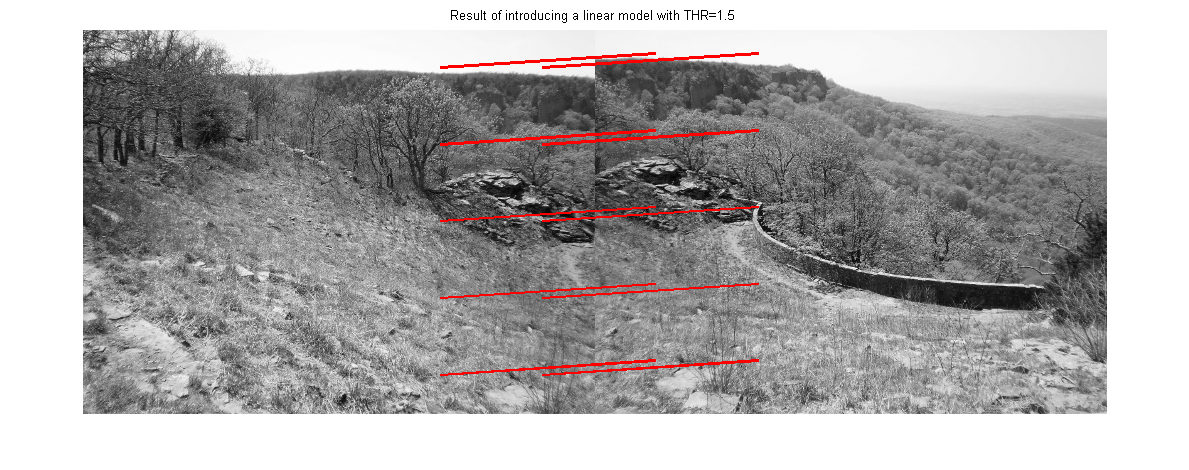
\includegraphics[width=\textwidth]{./img/ex1/matching_linear_model_15.png}
	\caption{Result of matching with THR=1.5 combined with linear model.}
	\label{fig:matching15lin}
\end{figure}

\begin{figure}[htb]
	\centering
		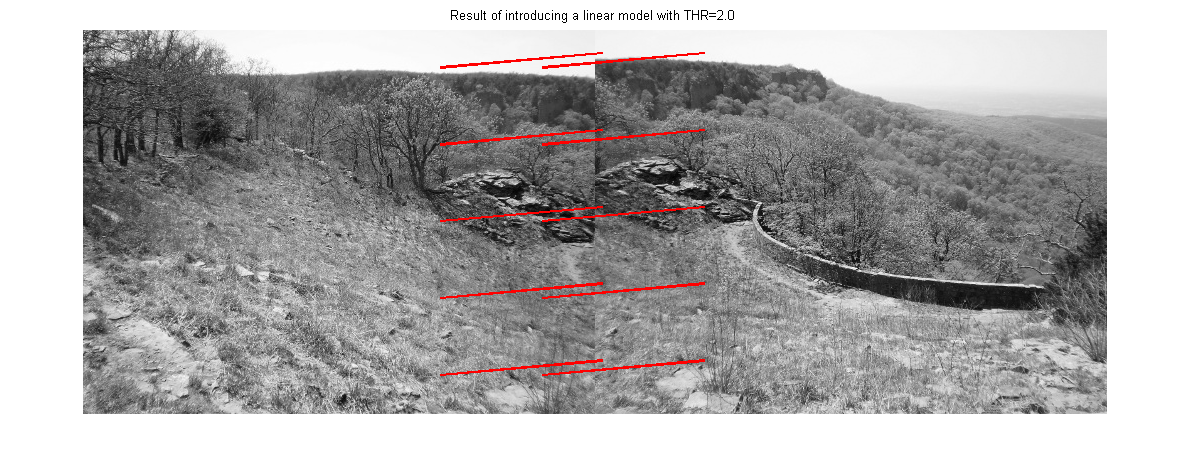
\includegraphics[width=\textwidth]{./img/ex1/matching_linear_model_20.png}
	\caption{Result of matching with THR=2.0 combined with linear model.}
	\label{fig:matching20lin}
\end{figure}

\begin{figure}[htb]
	\centering
		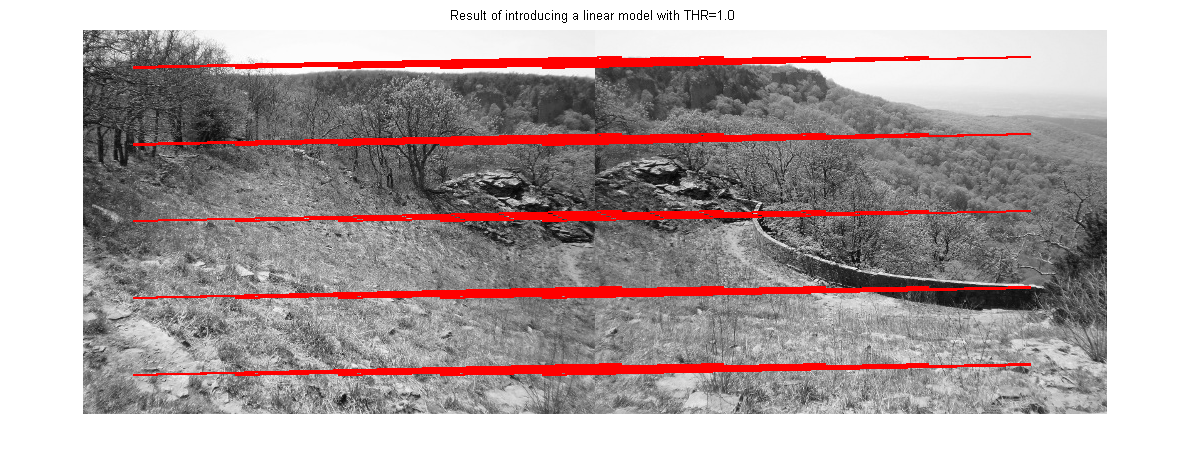
\includegraphics[width=\textwidth]{./img/ex1/matching_linear_model_10.png}
	\caption{Result of matching with THR=1.0 combined with linear model.}
	\label{fig:matching10lin}
\end{figure}

All things considered, the simple translational model seems to perform nicely for
the particular case of these two images as shown by the best of these three matches.
This is due to the fact that the difference between the two images can be seen
as a camera pan without significant rotation or skew. Therefore, the model
yields to good results.

\subsection{On the introduction of an afine model}

Figures \ref{fig:matching15afi}, \ref{fig:matching20afi} and \ref{fig:matching10afi}
show the result of combining with an afine model the matching results
obtained with thresholds 15, 20 and 10, respectively.

Much like in the previous case, and for the same causes, the best result is obtained
with THR=2.0 (figure \ref{fig:matching20afi}). However, while good, the result is
not much better than the (already good) results obtained in \ref{fig:matching20lin}.
On the other hand, the matches showed in figures \ref{fig:matching15afi} and \ref{fig:matching10afi}
are actually worse than those showed in figures \ref{fig:matching15lin} and
\ref{fig:matching10lin}. The reason behind this has already been posed in
the assignment's statement: the increase in the number of the model's DoF does not contribute
to a better match when there are many spurious correspondences. To this we add that
neither do these additional DoF contribute meaningfully when a good match can be found
with the adequate threshold and a simpler model.

\begin{figure}[htb]
	\centering
		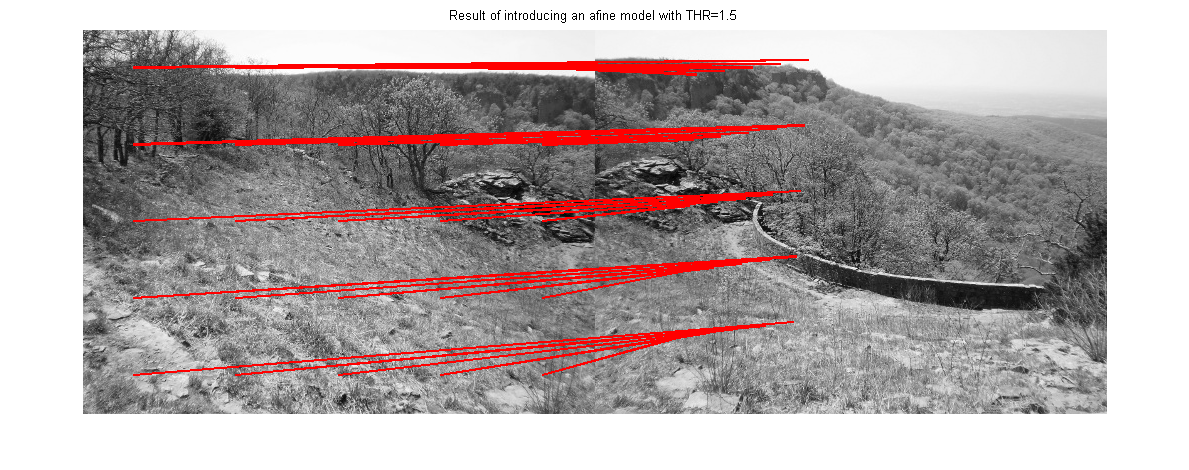
\includegraphics[width=\textwidth]{./img/ex1/matching_15_afine.png}
	\caption{Result of matching with THR=1.5 combined with afine model.}
	\label{fig:matching15afi}
\end{figure}

\begin{figure}[htb]
	\centering
		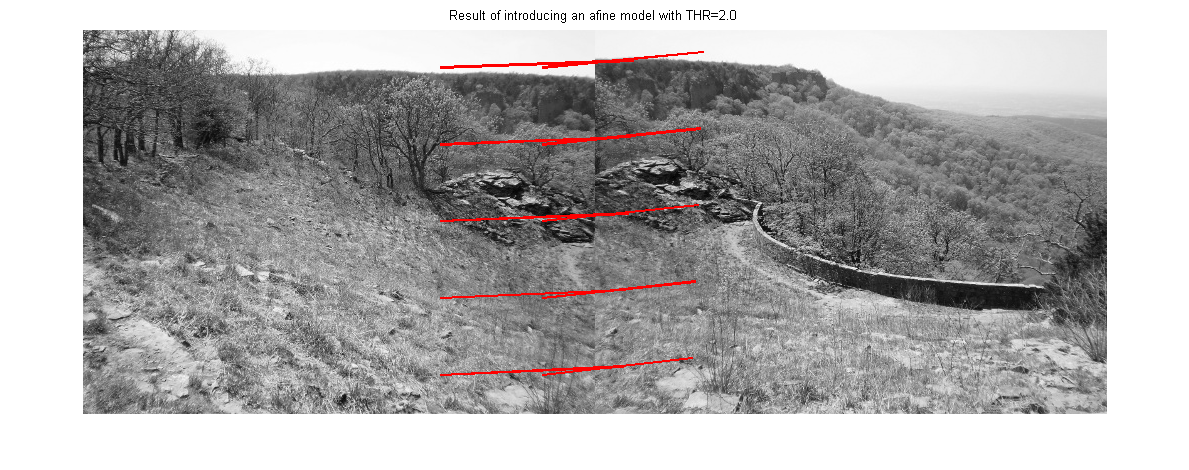
\includegraphics[width=\textwidth]{./img/ex1/matching_20_afine.png}
	\caption{Result of matching with THR=2.0 combined with afine model.}
	\label{fig:matching20afi}
\end{figure}

\begin{figure}[htb]
	\centering
		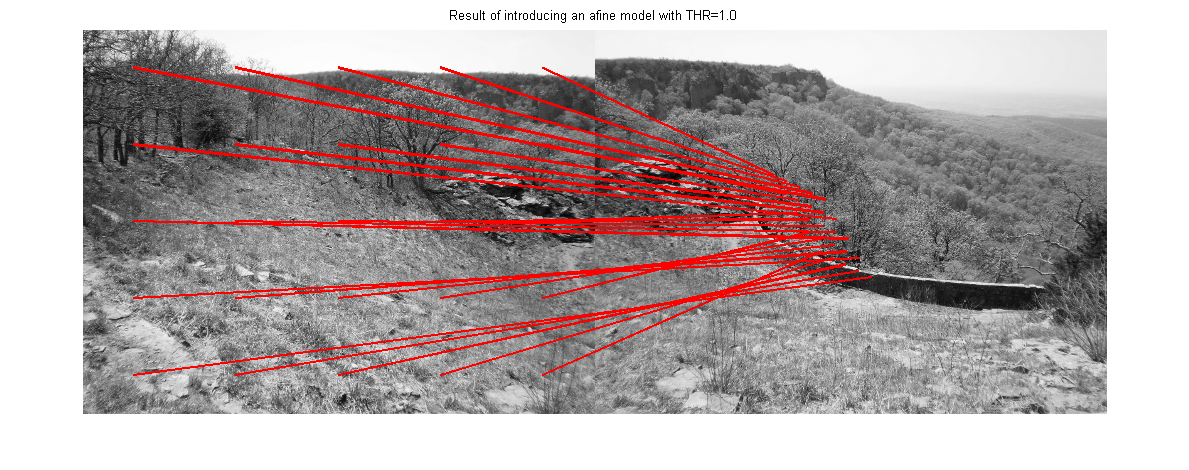
\includegraphics[width=\textwidth]{./img/ex1/matching_10_afine.png}
	\caption{Result of matching with THR=1.0 combined with afine model.}
	\label{fig:matching10afi}
\end{figure}

\subsection{Using a subset of with just the best matches}

Now we will analyze what happens when we select only the a subset with the
best matches to fit a model. From now on, we will deal exclusively with
the matches found with THR=1.5 since the following technique aims at
improving the fitting of the model even if an excess of matches
has been found due to a low threshold.

In figure \ref{fig:linearbest10} we can observe a very clear improvement over
the computed model in figure \ref{fig:matching15lin}. When we select only
the best matches, we are discarding the most spurious one. All in all this
leads to a much better result, comparable to that of figure
\ref{fig:matching20lin} (linear model after performing matching with THR=2.0).
Therefore, this technique help us to obtain good results even when we cannot
fine tune the THR parameter.

\begin{figure}[htb]
	\centering
		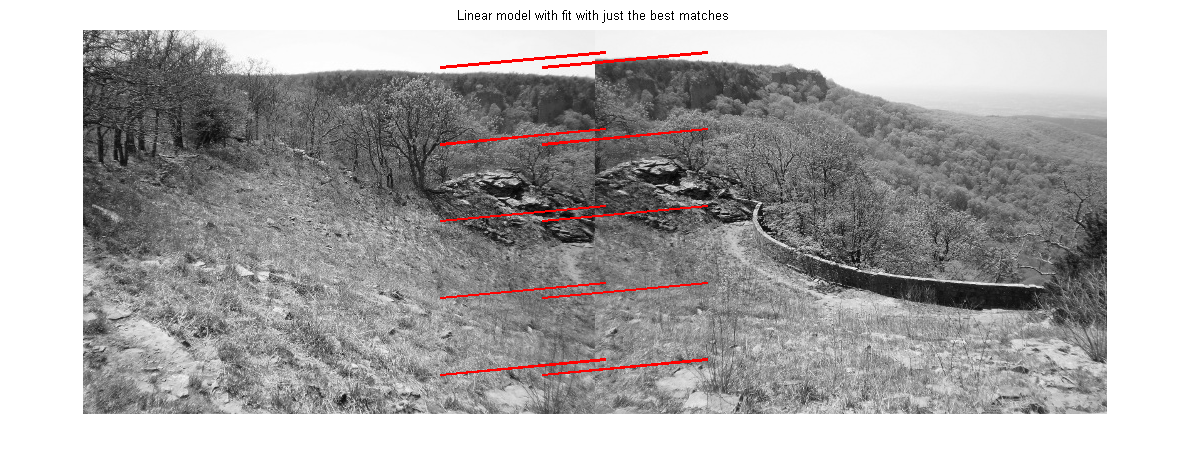
\includegraphics[width=\textwidth]{./img/ex1/linear_best_matches.png}
	\caption{Result of linear model using just the 10 best matches}
	\label{fig:linearbest10}
\end{figure}

In figure \ref{fig:afinebest10} we can observe the result of applying this same
technique with the afine model. We can see that the result is worse than before.
As the assignment's statement asserts, the least means square method is very
sensible to outliers when applied to the afine model. This can be seen when we
reduce the cardinality of the subset that we use to compute the model from 10 to
9. The result can be seen in figure \ref{fig:afinebest9}. This suggests that the
10th ``best'' match is actually an outlier which happens to have a low distance
between descriptors.

\begin{figure}[htb]
	\centering
		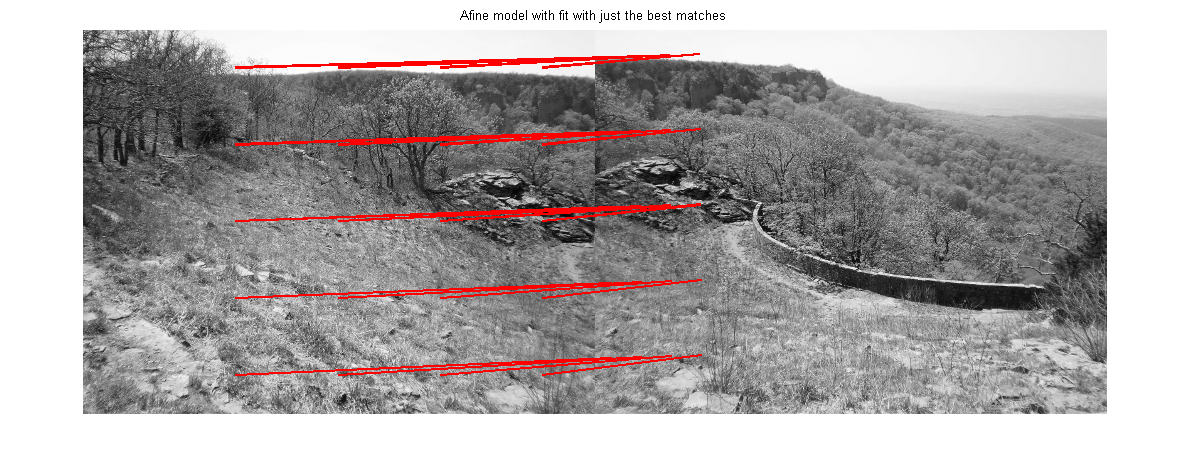
\includegraphics[width=\textwidth]{./img/ex1/afine_best_matches.png}
	\caption{Result of afine model using just the 10 best matches}
	\label{fig:afinebest10}
\end{figure}

\begin{figure}[htb]
	\centering
		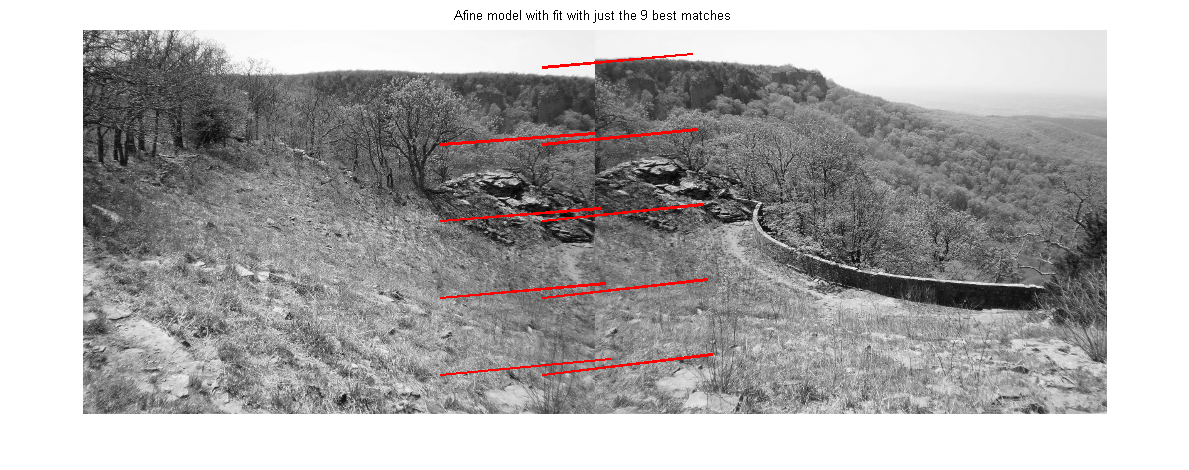
\includegraphics[width=\textwidth]{./img/ex1/afine_best_matches_9.png}
	\caption{Result of afine model using just the 9 best matches}
	\label{fig:afinebest9}
\end{figure}